% ============================================================================
% Chapter 4: Smart Contracts on Cardano
% Part of the Cardano Credential Verification Study Guide
% ============================================================================

\chapter{Smart Contracts on Cardano}
\label{ch:smart-contracts}

% --- TikZ styles for this chapter -------------------------------------------
\tikzset{
  guidebox/.style={draw, rounded corners=4pt, thick, align=center,
    font=\sffamily\small, fill=white, minimum height=1cm},
  guidearrow/.style={-{Latex[length=2.5mm]}, thick, color=gray!70!black},
  guidelabel/.style={font=\sffamily\footnotesize, text=gray!50!black},
}

Smart contracts are the enforcement layer of any blockchain-based system.
They are the reason a credential issued on Cardano is not merely a
database entry with a fancy name---they are what makes the credential
\emph{trustlessly verifiable}. In this chapter we build a complete
mental model of how Cardano smart contracts work, from the simplest
native scripts through full Plutus V2 validators, and then show exactly
how the credential system uses each type. By the end you will understand
why the system can guarantee that \emph{only} a licensed authority can
mint credential tokens, how multiple professionals can sign a work
product concurrently without conflicting, and how license validity can
be automatically linked to periodic dues payments.


% ============================================================================
\section{What is a Smart Contract?}
\label{sec:what-is-smart-contract}
% ============================================================================

\subsection{The Core Idea}

A smart contract is a piece of code that lives on a blockchain and
enforces rules automatically. Think of a vending machine: you insert
the correct amount of money and press a button, and the machine
dispenses the product. No cashier, no negotiation, no trust required.
The rules are mechanical. A smart contract is the digital equivalent---it
encodes rules in software that the blockchain itself enforces, removing
the need for any human intermediary to verify compliance.

In everyday life, a traditional contract says ``Party A agrees to pay
Party B \$100 on January 1st in exchange for Service X.'' Enforcement
depends on good faith, or failing that, a court. A smart contract
encodes the same logic in executable code: when the conditions are met,
the action happens automatically. When the conditions are \emph{not}
met, the action is rejected. There is no appeals process, no
bureaucratic delay, and no possibility of selective enforcement. The
code runs the same way for everyone.

\subsection{Cardano Validators Are Not Ethereum Smart Contracts}

This distinction is critical and trips up nearly everyone coming from
Ethereum. On Ethereum, a smart contract is a long-lived program with
its own persistent storage. You \emph{call functions} on it, it
updates its internal state, and it can call other contracts. It is
like a microservice that lives on the blockchain.

Cardano does not work this way.

On Cardano, a smart contract is a \textbf{validator}---a function that
receives some data and returns \texttt{True} or \texttt{False}. That is
it. The validator does not store state. It does not call other
validators. It does not have methods you invoke. It simply answers one
question: \emph{``Is this transaction allowed to spend this UTxO?''}

The best analogy is a bouncer at a nightclub. The bouncer does not own
the club. The bouncer does not manage the bar inventory. The bouncer
has exactly one job: check IDs at the door and decide ``yes, you may
enter'' or ``no, you may not.'' A Cardano validator is the bouncer for
a UTxO. When someone builds a transaction that tries to spend a UTxO
locked at a script address, the validator examines the transaction and
says ``yes'' or ``no.''

This design has profound consequences. Because validators are stateless
and pure---they examine inputs and produce a boolean---they are
\emph{deterministic}. The same inputs always produce the same output.
You can run the validator locally before submitting the transaction and
know with certainty whether it will succeed. There are no surprises
from concurrent state changes, no front-running attacks that alter the
execution path, and no gas estimation failures from state that changed
between simulation and execution.

\begin{figure}[H]
\centering
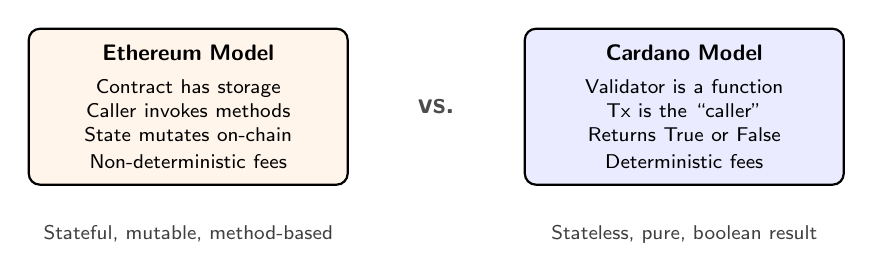
\begin{tikzpicture}[scale=0.9, every node/.style={transform shape}]
  % Ethereum side
  \node[guidebox, fill=orange!8, minimum width=4.5cm, minimum height=2.2cm,
    text width=4cm] (eth) at (-3.5,0) {
    \textbf{Ethereum Model}\\[4pt]
    \footnotesize Contract has storage\\
    \footnotesize Caller invokes methods\\
    \footnotesize State mutates on-chain\\
    \footnotesize Non-deterministic fees
  };
  % Cardano side
  \node[guidebox, fill=blue!8, minimum width=4.5cm, minimum height=2.2cm,
    text width=4cm] (ada) at (3.5,0) {
    \textbf{Cardano Model}\\[4pt]
    \footnotesize Validator is a function\\
    \footnotesize Tx is the ``caller''\\
    \footnotesize Returns True or False\\
    \footnotesize Deterministic fees
  };
  % VS
  \node[font=\sffamily\large\bfseries, text=gray!60!black] at (0,0) {vs.};
  % Labels
  \node[guidelabel] at (-3.5,-1.8) {Stateful, mutable, method-based};
  \node[guidelabel] at (3.5,-1.8) {Stateless, pure, boolean result};
\end{tikzpicture}
\caption{Ethereum's stateful contract model versus Cardano's stateless validator model. Cardano validators are pure functions that approve or reject UTxO spending.}
\label{fig:eth-vs-cardano}
\end{figure}

\subsection{Why This Matters for Credentials}

In the credential system, this design means that the minting policy for
license tokens is a validator that answers: ``Does this transaction
include a signature from the authorized licensing board?'' If yes,
minting proceeds. If no, the transaction is rejected by every node on
the network. There is no admin backdoor, no override function, and no
way to ``call'' the policy and ask it to mint tokens on your behalf.
The only path to minting is constructing a valid transaction that
satisfies the validator's conditions.


% ============================================================================
\section{Native Scripts (Phase 1)}
\label{sec:native-scripts}
% ============================================================================

\subsection{Overview}

Native scripts are Cardano's simplest form of smart contract. They
were introduced in the Shelley era and require no Plutus execution
engine---the ledger evaluates them directly during Phase 1 validation.
This means they incur \textbf{zero execution fees}. The only cost is
the standard transaction fee (${\sim}$0.17~ADA), making them ideal for
operations that need to happen frequently and cheaply.

Native scripts are built from five primitive building blocks. Each
block performs a simple check, and they can be combined to express
sophisticated conditions. Think of them as logic gates: each gate
checks one thing, and you wire them together to build the overall
access policy.

\subsection{The Five Script Types}

\subsubsection{ScriptPubkey: Single Key Requirement}

The simplest native script. It requires that the transaction includes a
signature from a specific verification key hash (public key hash). If
Alice's key hash is embedded in the script, then only a transaction
signed by Alice satisfies the script. This is the script type used for
the credential system's minting policies.

In the credential system, every authority wallet has a unique Ed25519
public key hash (PKH). The minting policy is a \texttt{ScriptPubkey}
containing that PKH. Any transaction that mints or burns tokens under
this policy must be signed by the authority's key. No one else on the
planet can produce a valid signature for that key, so no one else can
create or destroy credential tokens.

\subsubsection{ScriptAll: AND Logic}

Requires that \emph{all} listed conditions are satisfied. If the script
contains three sub-scripts, all three must pass. This is logical AND.

A practical example: a corporate account that requires signatures from
both the CEO and CFO. Neither can act alone. In the credential system,
\texttt{ScriptAll} is used when time-lock constraints are combined with
a key requirement---the authority's key \emph{and} the time constraint
must both be satisfied.

\subsubsection{ScriptAny: OR Logic}

Requires that \emph{at least one} listed condition is satisfied. If the
script contains three sub-scripts, any single one passing is sufficient.
This is logical OR.

A practical example: a recovery mechanism where either the primary key
or a backup key can authorize a transaction. If you lose your primary
key, the backup still works.

\subsubsection{ScriptNofK: Threshold (N-of-K)}

Requires that at least $N$ out of $K$ listed conditions are satisfied.
This generalizes both \texttt{ScriptAll} ($N = K$) and \texttt{ScriptAny}
($N = 1$). A 3-of-5 multi-signature governance scheme uses
\texttt{ScriptNofK} with $N = 3$ and $K = 5$.

This is particularly relevant for the credential system's future
governance upgrade path. Instead of a single authority key controlling
minting, a \texttt{ScriptNofK} policy could require signatures from
3~of~5 board members, distributing trust and eliminating single-key
centralization risk.

\subsubsection{TimeLock: Temporal Constraints}

Two time-lock primitives restrict \emph{when} a script is valid:
\begin{itemize}[nosep]
  \item \textbf{InvalidBefore} (also called \texttt{TimelockStart}):
    the transaction is invalid before a specified slot number. The
    script cannot be satisfied until that slot has passed.
  \item \textbf{InvalidHereAfter} (also called \texttt{TimelockExpiry}):
    the transaction is invalid at or after a specified slot number. The
    script can only be satisfied before that slot.
\end{itemize}

Time locks are used in the credential system to create minting policies
that expire. For example, an authority might create a policy that can
only mint tokens during a specific fiscal year. After the expiry slot,
no new tokens can be minted under that policy, even by the authority.
This provides a cryptographic guarantee that the token supply is frozen
after a certain point.

\begin{figure}[H]
\centering
\begin{tikzpicture}[scale=0.85, every node/.style={transform shape}]
  % ScriptPubkey
  \node[guidebox, fill=blue!8, minimum width=3.6cm, minimum height=1.4cm]
    (pk) at (-3.8,4.5)
    {\textbf{ScriptPubkey}\\[2pt]\footnotesize Requires key $K_1$};
  \node[guidelabel] at (-3.8,3.4) {Single signature gate};

  % ScriptAll
  \node[guidebox, fill=green!8, minimum width=3.6cm, minimum height=1.8cm,
    text width=3.2cm] (all) at (1,4.5) {
    \textbf{ScriptAll (AND)}\\[2pt]
    \footnotesize $K_1$ \textbf{and} $K_2$ \textbf{and} $K_3$\\
    \footnotesize All must sign
  };
  \node[guidelabel] at (1,3.15) {All conditions required};

  % ScriptAny
  \node[guidebox, fill=orange!8, minimum width=3.6cm, minimum height=1.8cm,
    text width=3.2cm] (any) at (5.8,4.5) {
    \textbf{ScriptAny (OR)}\\[2pt]
    \footnotesize $K_1$ \textbf{or} $K_2$ \textbf{or} $K_3$\\
    \footnotesize Any one suffices
  };
  \node[guidelabel] at (5.8,3.15) {One condition sufficient};

  % ScriptNofK
  \node[guidebox, fill=purple!8, minimum width=3.6cm, minimum height=1.8cm,
    text width=3.2cm] (nofk) at (-3.8,1.2) {
    \textbf{ScriptNofK}\\[2pt]
    \footnotesize $N$-of-$K$ threshold\\
    \footnotesize e.g.\ 3-of-5 multi-sig
  };
  \node[guidelabel] at (-3.8,-0.15) {Threshold gate};

  % TimeLock
  \node[guidebox, fill=yellow!8, minimum width=7.2cm, minimum height=1.8cm,
    text width=6.8cm] (time) at (3.4,1.2) {
    \textbf{TimeLock}\\[2pt]
    \footnotesize \texttt{InvalidBefore(slot)}: not valid until slot $S_1$\\
    \footnotesize \texttt{InvalidHereAfter(slot)}: not valid at or after slot $S_2$
  };
  \node[guidelabel] at (3.4,-0.15) {Temporal window constraints};

  % Composition example
  \node[guidebox, fill=gray!10, minimum width=10.6cm, minimum height=1.6cm,
    text width=10cm] (combo) at (1,-1.8) {
    \textbf{Credential Minting Policy (Combined)}\\[2pt]
    \footnotesize \texttt{ScriptAll}(\texttt{ScriptPubkey}($K_{\mathrm{authority}}$),
    \texttt{InvalidHereAfter}($S_{\mathrm{expiry}}$))\\
    \footnotesize Authority key required AND must be before expiry slot
  };

  % Arrows to combo
  \draw[guidearrow, dashed] (pk.south) -- ++(0,-0.6) -| (combo.north west);
  \draw[guidearrow, dashed] (time.south) -- ++(0,-0.3) -| (combo.north east);
\end{tikzpicture}
\caption{The five native script types and how they compose. The credential system's minting policy typically combines a \texttt{ScriptPubkey} (authority key) with an optional \texttt{InvalidHereAfter} (time lock) inside a \texttt{ScriptAll} wrapper.}
\label{fig:native-scripts}
\end{figure}

\subsection{Why Native Scripts for Minting Policies?}

The credential system deliberately uses native scripts---not Plutus
validators---for its minting policies. The reason is economics. A
native script minting transaction costs approximately 0.17~ADA with
zero execution fees. A Plutus V2 minting transaction costs 0.3--0.5~ADA
because the Plutus execution engine must evaluate the script, consuming
CPU steps and memory units that are priced into the fee.

For a system that might mint thousands of credential tokens (one license
NFT per professional, plus signature tokens and validity tokens), the
difference compounds. At 10,000 licenses with associated tokens, native
scripts save approximately 1,300--3,300~ADA compared to Plutus-based
minting policies. The trade-off is expressiveness: native scripts can
only check keys and time constraints, while Plutus scripts can examine
the full transaction. For minting policies where the rule is simply
``the authority must sign,'' native scripts provide the same security
guarantee at a fraction of the cost.


% ============================================================================
\section{Plutus V2 Validators (Phase 2)}
\label{sec:plutus-v2}
% ============================================================================

\subsection{Beyond Simple Scripts}

Native scripts answer simple questions: ``Is this key present?'' ``Is
it before slot X?'' But many operations require examining the
\emph{content} of a transaction---which tokens are being moved, what
data is attached, how much ADA is being paid to whom. For these
operations, Cardano provides Plutus validators: full-powered smart
contracts written in Haskell (compiled to Plutus Core, which runs on
the Untyped Plutus Lambda Calculus---UPLC) and evaluated during
Phase~2 validation.

Plutus V2, introduced in the Vasil hard fork (September 2022), added
three features critical for the credential system:
\begin{itemize}[nosep]
  \item \textbf{Reference Inputs (CIP-31)}: read a UTxO without
    consuming it. This lets verifiers inspect credential metadata
    without spending the token.
  \item \textbf{Inline Datums (CIP-32)}: attach data directly to a
    UTxO output instead of storing only a datum hash. This eliminates
    the need to look up datums separately.
  \item \textbf{Reference Scripts (CIP-33)}: reference a script stored
    in a UTxO rather than including the script in every transaction.
    This reduces transaction sizes significantly.
\end{itemize}

\subsection{The Three Inputs to a Validator}

Every Plutus V2 validator receives exactly three pieces of information
when evaluating whether a UTxO can be spent. Understanding these three
inputs is the key to understanding all Cardano smart contracts.

\subsubsection{Datum: The State}

The \textbf{datum} is data attached to the UTxO being spent. Think of
it as a note taped to a locked box. When someone created the UTxO and
sent tokens to the script address, they included this datum to record
the state or context of that particular UTxO.

In the credential system, the \texttt{SignerDatum} is attached to each
signer's deposit UTxO. It records the signer's public key hash, the
SHA-256 hash of the document being signed, the slot at which the
deposit was made, the policy IDs of the signature and validity tokens,
and the validity token's expiry slot. This datum is the ``evidence
packet'' that proves who signed, what they signed, and when.

\subsubsection{Redeemer: The Action}

The \textbf{redeemer} is data provided by the transaction that wants to
spend the UTxO. Think of it as the instruction or request. The datum
says ``here is what was stored.'' The redeemer says ``here is what I
want to do with it.''

In the credential system, the redeemer is an integer discriminator that
tells the validator which action is being performed: \texttt{COLLECT}
(redeemer~0), \texttt{FINALIZE} (redeemer~1), or \texttt{RECLAIM}
(redeemer~2). Each action triggers different validation logic inside the
validator.

\subsubsection{Script Context: The Transaction}

The \textbf{script context} is the full transaction being validated---all
inputs, all outputs, all signatures, all minted tokens, all time
constraints, everything. The validator can inspect any part of the
transaction to make its decision.

This is what gives Plutus validators their power compared to native
scripts. A native script can only check ``is this key present?'' A
Plutus validator can check ``does this transaction include an output
paying exactly 50~ADA to the authority's address?'' or ``does this
transaction mint exactly one token under policy XYZ?''

The validator examines all three inputs---datum, redeemer, and script
context---and returns \texttt{True} (the UTxO may be spent, the
transaction is valid) or \texttt{False} (the spending is rejected, the
transaction fails).

\begin{figure}[H]
\centering
\begin{tikzpicture}[scale=0.88, every node/.style={transform shape}]
  % Datum box
  \node[guidebox, fill=blue!8, minimum width=3.8cm, minimum height=2.0cm,
    text width=3.4cm] (datum) at (-4,2.5) {
    \textbf{Datum}\\[3pt]
    \footnotesize ``The State''\\[2pt]
    \footnotesize Data attached to\\the UTxO at creation\\[2pt]
    \scriptsize\textit{SignerDatum:}\\
    \scriptsize signer\_pkh,\\
    \scriptsize document\_hash,\\
    \scriptsize deposit\_slot, ...
  };

  % Redeemer box
  \node[guidebox, fill=green!8, minimum width=3.8cm, minimum height=2.0cm,
    text width=3.4cm] (redeemer) at (0,2.5) {
    \textbf{Redeemer}\\[3pt]
    \footnotesize ``The Action''\\[2pt]
    \footnotesize Data provided by\\the spending tx\\[2pt]
    \scriptsize\textit{CollectRedeemer (0)}\\
    \scriptsize\textit{FinalizeRedeemer (1)}\\
    \scriptsize\textit{ReclaimRedeemer (2)}
  };

  % ScriptContext box
  \node[guidebox, fill=orange!8, minimum width=3.8cm, minimum height=2.0cm,
    text width=3.4cm] (ctx) at (4,2.5) {
    \textbf{Script Context}\\[3pt]
    \footnotesize ``The Transaction''\\[2pt]
    \footnotesize All inputs, outputs,\\signatures, mints,\\time bounds, fees
  };

  % Validator
  \node[guidebox, fill=purple!8, minimum width=6cm, minimum height=1.4cm,
    text width=5.5cm] (val) at (0,-0.3) {
    \textbf{Plutus V2 Validator}\\[3pt]
    \footnotesize \texttt{validator(datum, redeemer, ctx) -> Bool}
  };

  % Result
  \node[guidebox, fill=green!8, minimum width=2.2cm] (yes) at (-2.5,-2.5) {
    \textbf{True}\\[2pt]\footnotesize Spend allowed
  };
  \node[guidebox, fill=red!6, minimum width=2.2cm] (no) at (2.5,-2.5) {
    \textbf{False}\\[2pt]\footnotesize Spend rejected
  };

  % Arrows in
  \draw[guidearrow] (datum.south) -- (val.north -| datum.south);
  \draw[guidearrow] (redeemer.south) -- (val.north);
  \draw[guidearrow] (ctx.south) -- (val.north -| ctx.south);

  % Arrows out
  \draw[guidearrow, color=green!60!black] (val.south west) ++(0.5,0)
    -- (yes.north);
  \draw[guidearrow, color=red!60!black] (val.south east) ++(-0.5,0)
    -- (no.north);
\end{tikzpicture}
\caption{The three inputs to a Plutus V2 validator. The validator function receives the datum (state stored with the UTxO), the redeemer (action requested by the spending transaction), and the script context (the full transaction), and returns a boolean.}
\label{fig:plutus-validator}
\end{figure}

\subsection{Deterministic Execution}

One of Cardano's most important properties is that Plutus execution is
\textbf{deterministic}. Because the validator is a pure function of its
three inputs, and because the eUTxO model means the inputs are known
before the transaction is submitted, you can run the validator locally
and know \emph{exactly} what will happen on-chain. The fee is
calculable in advance. The result is predictable. There are no
surprises.

This stands in stark contrast to Ethereum, where a transaction can fail
at execution time because another transaction altered the contract's
state between when you simulated it and when it was included in a
block. On Cardano, if the validator succeeds locally, it will succeed
on-chain (assuming the UTxOs have not been spent by another transaction
in the interim---but that is a concurrency issue the eUTxO model makes
explicit, not a hidden state-mutation surprise).


% ============================================================================
\section{Execution Units (exUnits)}
\label{sec:exunits}
% ============================================================================

\subsection{CPU Steps and Memory Units}

Every Plutus script execution consumes two budgeted resources:
\textbf{CPU steps} and \textbf{memory units}. CPU steps measure
computational complexity---how many operations the validator performs.
Memory units measure how much memory the validator allocates during
execution. Both are metered precisely by the UPLC evaluator.

Each transaction has a maximum execution budget, currently set at
10~billion CPU steps and 10~million memory units per transaction (with
per-script limits as well). If a validator exceeds either limit, the
transaction fails. The transaction builder calculates the exact
execution cost before submission, so you know whether you will exceed
the budget before spending any ADA.

\subsection{How exUnits Affect Fees}

Transaction fees on Cardano follow a linear formula:
\[
  \mathrm{fee} = a \times \mathrm{size\_bytes} + b + c_{\mathrm{cpu}} \times \mathrm{cpu\_steps} + c_{\mathrm{mem}} \times \mathrm{mem\_units}
\]
where $a$ and $b$ are the base fee parameters (currently $a = 44$
lovelace per byte, $b = 155{,}381$ lovelace), and $c_{\mathrm{cpu}}$
and $c_{\mathrm{mem}}$ are the execution fee coefficients.

For native scripts, the execution terms ($c_{\mathrm{cpu}}$ and
$c_{\mathrm{mem}}$) are zero---native scripts are evaluated by the
ledger rules themselves, not by the Plutus execution engine. This is
why native script transactions cost ${\sim}$0.17~ADA: only the
size-based fee applies.

For Plutus V2 transactions, the execution terms add 0.1--0.3~ADA
depending on script complexity, bringing the total to ${\sim}$0.3--0.5~ADA.
This is still dramatically cheaper than Ethereum (where gas costs can
reach \$1--\$15+ for contract interactions), but it is a measurable
difference when multiplied across thousands of transactions.

\subsection{Deterministic Cost Estimation}

Because Plutus execution is deterministic, the cost is known
\emph{before} the transaction is submitted to the network. The
transaction builder runs the validator against the exact inputs,
records the CPU and memory consumption, embeds the exUnits in the
transaction, and calculates the precise fee. If the fee changes between
estimation and submission, it is because a UTxO was spent (a
concurrency event), not because the validator behaved differently.

\begin{figure}[H]
\centering
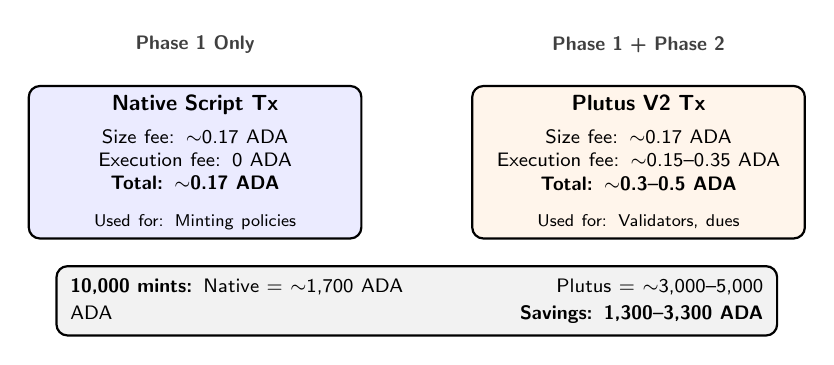
\begin{tikzpicture}[scale=0.88, every node/.style={transform shape}]
  % Native Script
  \node[guidebox, fill=blue!8, minimum width=4.8cm, minimum height=2.2cm,
    text width=4.4cm] (native) at (-3.2,0) {
    \textbf{Native Script Tx}\\[4pt]
    \footnotesize Size fee: ${\sim}$0.17 ADA\\
    \footnotesize Execution fee: 0 ADA\\
    \footnotesize \textbf{Total: ${\sim}$0.17 ADA}\\[4pt]
    \scriptsize Used for: Minting policies
  };

  % Plutus V2
  \node[guidebox, fill=orange!8, minimum width=4.8cm, minimum height=2.2cm,
    text width=4.4cm] (plutus) at (3.2,0) {
    \textbf{Plutus V2 Tx}\\[4pt]
    \footnotesize Size fee: ${\sim}$0.17 ADA\\
    \footnotesize Execution fee: ${\sim}$0.15--0.35 ADA\\
    \footnotesize \textbf{Total: ${\sim}$0.3--0.5 ADA}\\[4pt]
    \scriptsize Used for: Validators, dues
  };

  % Labels
  \node[guidelabel, font=\sffamily\footnotesize\bfseries]
    at (-3.2,1.7) {Phase 1 Only};
  \node[guidelabel, font=\sffamily\footnotesize\bfseries]
    at (3.2,1.7) {Phase 1 + Phase 2};

  % Cost comparison bar
  \node[guidebox, fill=gray!10, minimum width=10.4cm, minimum height=1.0cm,
    text width=10cm] at (0,-2.0) {
    \footnotesize \textbf{10,000 mints:} Native = ${\sim}$1,700 ADA
    \hfill Plutus = ${\sim}$3,000--5,000 ADA
    \hfill \textbf{Savings: 1,300--3,300 ADA}
  };
\end{tikzpicture}
\caption{Fee comparison between native script and Plutus V2 transactions. Native scripts avoid Phase~2 execution costs entirely, making them the economical choice for simple minting policies.}
\label{fig:exunits}
\end{figure}


% ============================================================================
\section{Minting Policies}
\label{sec:minting-policies}
% ============================================================================

\subsection{What is a Minting Policy?}

A minting policy is a special type of validator that controls the
creation (minting) and destruction (burning) of native tokens. On
Cardano, every native token belongs to a \textbf{policy ID}, which is
the Blake2b-224 hash of the minting policy script. The policy ID is
the token's identity---it tells you \emph{which rules govern this
token's existence}.

This is fundamentally different from Ethereum, where token contracts
are long-lived programs that maintain a balance mapping. On Cardano,
tokens are ledger-level assets. The minting policy only runs when
tokens are created or destroyed. Transfers between wallets require no
script execution at all---they are plain UTxO transactions, just like
sending ADA.

\subsection{Policy ID = Script Hash}

The policy ID is computed deterministically:
\[
  \mathrm{PolicyID} = \mathrm{Blake2b}_{224}(\mathrm{CBOR}(\mathrm{script}))
\]
Because the hash is deterministic, anyone can independently verify that
a given policy ID corresponds to a specific script. If the script says
``only Alice's key can mint,'' and you verify the script hash matches
the policy ID, then you know with mathematical certainty that only
Alice can have minted those tokens. No trust required. No authority to
query. Just hash verification.

\subsection{The Credential System's Minting Policy}

In the credential system, the minting policy is a \texttt{ScriptPubkey}
native script containing the authority's public key hash. The
\texttt{PlutusV2MintingPolicy} class (despite its name, it uses native
scripts for economic efficiency) constructs this policy:

\begin{enumerate}[nosep]
  \item The authority's 28-byte Ed25519 verification key hash is
    embedded in a \texttt{ScriptPubkey} native script.
  \item Optionally, time-lock constraints are added via
    \texttt{ScriptAll} (combining the key requirement with
    \texttt{InvalidBefore}/\texttt{InvalidHereAfter}).
  \item The policy ID is the Blake2b-224 hash of the CBOR-serialized
    script.
  \item The policy is saved as both a JSON metadata file and a CBOR
    binary for transaction building.
\end{enumerate}

This means \textbf{only the authority can mint or burn credential
tokens}. A transaction attempting to mint tokens under this policy must
include a valid Ed25519 signature from the authority's private key.
Without that key, no entity---not even Cardano node operators or stake
pool operators---can create tokens under that policy.

\begin{figure}[H]
\centering
\begin{tikzpicture}[scale=0.88, every node/.style={transform shape}]
  % Authority key
  \node[guidebox, fill=blue!8, minimum width=4cm, minimum height=1.2cm]
    (key) at (0,3.5) {
    \textbf{Authority Key}\\[2pt]
    \footnotesize PKH: 28-byte Ed25519 hash
  };

  % ScriptPubkey
  \node[guidebox, fill=green!8, minimum width=4cm, minimum height=1.2cm]
    (script) at (0,1.8) {
    \textbf{ScriptPubkey(PKH)}\\[2pt]
    \footnotesize Native script embedding PKH
  };

  % CBOR + Hash
  \node[guidebox, fill=yellow!8, minimum width=4cm, minimum height=1.2cm]
    (hash) at (0,0.1) {
    \textbf{Blake2b-224(CBOR(script))}\\[2pt]
    \footnotesize Produces 28-byte Policy ID
  };

  % Policy ID
  \node[guidebox, fill=purple!8, minimum width=6cm, minimum height=1.2cm]
    (pid) at (0,-1.6) {
    \textbf{Policy ID}\\[2pt]
    \footnotesize \texttt{a1b2c3d4...} (56 hex chars)\\
    \footnotesize Uniquely identifies all tokens minted by this authority
  };

  % Tokens
  \node[guidebox, fill=orange!8, minimum width=2.4cm] (t1) at (-3.5,-3.5)
    {\footnotesize License NFTs};
  \node[guidebox, fill=orange!8, minimum width=2.4cm] (t2) at (0,-3.5)
    {\footnotesize Sig Tokens};
  \node[guidebox, fill=orange!8, minimum width=2.4cm] (t3) at (3.5,-3.5)
    {\footnotesize Val Tokens};

  % Arrows
  \draw[guidearrow] (key) -- (script);
  \draw[guidearrow] (script) -- (hash);
  \draw[guidearrow] (hash) -- (pid);
  \draw[guidearrow] (pid.south) -- ++(0,-0.3) -| (t1.north);
  \draw[guidearrow] (pid.south) -- (t2.north);
  \draw[guidearrow] (pid.south) -- ++(0,-0.3) -| (t3.north);
\end{tikzpicture}
\caption{Minting policy derivation: the authority's key hash is embedded in a native script, which is hashed to produce the deterministic Policy ID that governs all credential tokens.}
\label{fig:minting-policy}
\end{figure}

\subsection{Verification Without Trust}

A verifier who wants to confirm that a credential token is legitimate
performs these steps:
\begin{enumerate}[nosep]
  \item Look up the token's policy ID on-chain.
  \item Check that the policy ID is in the registry of known
    authorities (e.g., ``Policy ID \texttt{abc123...} belongs to the
    California Board of Professional Engineers'').
  \item The mathematical relationship between the policy ID and the
    authority's key guarantees that only the authority could have minted
    that token.
\end{enumerate}

No API call to the licensing board. No database query. No waiting for
business hours. The verification is a deterministic mathematical
operation that takes milliseconds.


% ============================================================================
\section{The SignatureCollectionValidator}
\label{sec:signature-collection-validator}
% ============================================================================

\subsection{The Problem: Multi-Party Signing on eUTxO}

The Signature Collection Validator is the most complex and most
important smart contract in the credential system. It solves a problem
that is conceptually simple---collect signatures from multiple
professionals on a single document---but technically challenging on
Cardano's eUTxO model.

The challenge is \textbf{concurrency}. On Ethereum, multiple users can
call the same contract simultaneously because the contract maintains
internal state (a mapping of who has signed). The EVM serializes these
calls and updates the state sequentially. On Cardano's eUTxO model,
there is no shared mutable state. A UTxO can only be spent once. If
two signers try to spend the same UTxO at the same time, one
transaction succeeds and the other fails.

Consider a naive design: a single UTxO at the script address holds the
``work product state'' (which signers have signed so far). Signer~A
builds a transaction that spends this UTxO and creates a new one with
their signature added. Signer~B, working simultaneously, builds a
transaction that also spends the \emph{same original UTxO}. Both
transactions cannot succeed---the first one to be included in a block
wins, and the second fails because the UTxO it references no longer
exists. This is the eUTxO concurrency bottleneck.

\subsection{The Solution: Independent Per-Signer UTxOs}

The credential system's \texttt{SignatureCollectionValidator} solves
this elegantly: instead of maintaining a single shared-state UTxO,
\textbf{each signer creates their own independent UTxO} at the script
address. There is no shared state to contend over. Signer~A deposits
their tokens into one UTxO. Signer~B deposits their tokens into a
different UTxO. Both UTxOs sit at the same script address but are
completely independent. They can be created in the same block, in
different blocks, or even simultaneously---there is zero contention.

Think of it like a suggestion box with individual envelopes. Instead of
everyone writing on the same sheet of paper (which creates a queue),
each person drops their own sealed envelope into the box. The envelopes
do not interfere with each other. When the authority is ready to
finalize, they open all the envelopes at once.

\subsection{The Three Redeemer Actions}

The validator supports three actions, identified by their
\texttt{CONSTR\_ID} discriminator:

\subsubsection{COLLECT (Redeemer 0)}

The \texttt{CollectRedeemer} (constructor ID~0) is used when a signer
deposits their tokens. Any required signer can submit a transaction
that:
\begin{enumerate}[nosep]
  \item Creates a new UTxO at the validator's script address.
  \item Attaches a \texttt{SignerDatum} containing their PKH, the
    document hash, the deposit slot, the policy IDs of their signature
    and validity tokens, and the validity expiry slot.
  \item Includes at least one signature token and one validity token in
    the UTxO's value.
  \item Is signed by the signer's private key (proving ownership of the
    PKH in the datum).
\end{enumerate}

The validator checks that:
\begin{itemize}[nosep]
  \item The signer's PKH is in the list of required signers.
  \item The signer has not already deposited (no duplicate deposits).
  \item The validity token has not expired (expiry slot is in the
    future relative to the current slot).
  \item If a validity deadline is set, the expiry slot does not exceed
    it.
  \item The required tokens (signature token + validity token) are
    present in the UTxO value.
\end{itemize}

This is the critical concurrency-safe operation. Because each
\texttt{COLLECT} creates a \emph{new, independent} UTxO rather than
modifying an existing one, multiple signers can deposit simultaneously
without any risk of transaction collision. Signer~1 in New York and
Signer~2 in Los Angeles can submit their deposit transactions at the
exact same second, and both will succeed because they are creating
different UTxOs, not competing to spend the same one.

\subsubsection{FINALIZE (Redeemer 1)}

The \texttt{FinalizeRedeemer} (constructor ID~1) is used by the
authority to complete the signing process. When all required signers
have deposited their tokens, the authority builds a single transaction
that:
\begin{enumerate}[nosep]
  \item Consumes \emph{all} per-signer UTxOs at the script address as
    inputs (one input per signer).
  \item Creates a single output containing all collected tokens.
  \item Must be signed by the authority's key.
  \item Includes the \texttt{FinalizeRedeemer} for each script input.
\end{enumerate}

This is an \textbf{atomic sweep}: all per-signer deposits are consumed
in a single transaction. Either the finalization succeeds entirely (all
UTxOs are spent and the work product is complete) or it fails entirely
(no UTxOs are spent). There is no partial finalization.

The validator checks that:
\begin{itemize}[nosep]
  \item The transaction is signed by the authority's PKH.
  \item All required signers have deposits present among the inputs.
  \item The document hash in each \texttt{SignerDatum} matches the work
    product's document hash.
\end{itemize}

\subsubsection{RECLAIM (Redeemer 2)}

The \texttt{ReclaimRedeemer} (constructor ID~2) is the escape hatch. If
a work product is cancelled before finalization, signers need a way to
recover their deposited tokens. A signer can submit a reclaim
transaction that:
\begin{enumerate}[nosep]
  \item Consumes their specific UTxO at the script address.
  \item Returns their signature token and validity token to their wallet.
  \item Must be signed by the same key that made the original deposit
    (the signer's PKH in the \texttt{SignerDatum}).
\end{enumerate}

The validator checks that the transaction signer matches the
\texttt{signer\_pkh} in the datum. Only the original depositor can
reclaim their tokens---no one else, not even the authority, can spend a
signer's deposit UTxO via the \texttt{RECLAIM} action.

\subsection{The SignerDatum}

Each deposit UTxO carries a \texttt{SignerDatum}, which is a Plutus
data type (\texttt{PlutusData} subclass with \texttt{CONSTR\_ID = 0})
containing six fields:

\begin{table}[H]
\centering
\small
\begin{tabular}{@{}llp{6.5cm}@{}}
\toprule
\textbf{Field} & \textbf{Type} & \textbf{Description} \\
\midrule
\texttt{signer\_pkh} & \texttt{bytes} & 28-byte public key hash of the signer \\
\texttt{document\_hash} & \texttt{bytes} & SHA-256 hash of the document being signed \\
\texttt{deposit\_slot} & \texttt{int} & Cardano slot number at deposit time \\
\texttt{sig\_token\_policy} & \texttt{bytes} & Policy ID of the signature token \\
\texttt{val\_token\_policy} & \texttt{bytes} & Policy ID of the validity token \\
\texttt{validity\_expiry\_slot} & \texttt{int} & Slot at which the validity token expires \\
\bottomrule
\end{tabular}
\caption{SignerDatum fields. Each deposit UTxO at the validator address carries this datum, creating a complete evidence record for each signer.}
\label{tab:signer-datum}
\end{table}

This datum serves as the on-chain evidence record. After finalization,
anyone can read the datum from the consumed UTxOs (via transaction
history) and independently verify: \emph{who} signed (signer\_pkh),
\emph{what} they signed (document\_hash), \emph{when} they signed
(deposit\_slot), \emph{under what authority} (token policy IDs), and
\emph{whether their credential was valid} at signing time
(validity\_expiry\_slot $>$ deposit\_slot).

\subsection{Concurrency in Detail: The COLLECT $\rightarrow$ FINALIZE Flow}

Let us trace through a concrete example with three signers---Alice
(a structural engineer), Bob (a geotechnical engineer), and Carol
(the project manager)---signing off on a seismic retrofit design.

\begin{figure}[H]
\centering
\begin{tikzpicture}[scale=0.78, every node/.style={transform shape}]
  % Actors
  \node[guidebox, fill=blue!8, minimum width=1.8cm, minimum height=0.7cm,
    font=\sffamily\footnotesize] (alice) at (0,0) {Alice};
  \node[guidebox, fill=green!8, minimum width=1.8cm, minimum height=0.7cm,
    font=\sffamily\footnotesize] (bob) at (3.5,0) {Bob};
  \node[guidebox, fill=orange!8, minimum width=1.8cm, minimum height=0.7cm,
    font=\sffamily\footnotesize] (carol) at (7,0) {Carol};
  \node[guidebox, fill=purple!8, minimum width=1.8cm, minimum height=0.7cm,
    font=\sffamily\footnotesize] (val) at (10.5,0) {Validator};
  \node[guidebox, fill=gray!10, minimum width=1.8cm, minimum height=0.7cm,
    font=\sffamily\footnotesize] (auth) at (14,0) {Authority};

  % Lifelines
  \draw[dashed, gray!40] (0,-0.5) -- (0,-14.5);
  \draw[dashed, gray!40] (3.5,-0.5) -- (3.5,-14.5);
  \draw[dashed, gray!40] (7,-0.5) -- (7,-14.5);
  \draw[dashed, gray!40] (10.5,-0.5) -- (10.5,-14.5);
  \draw[dashed, gray!40] (14,-0.5) -- (14,-14.5);

  % Phase 1: Setup
  \node[guidelabel, font=\sffamily\footnotesize\bfseries, text=gray!70!black,
    anchor=west] at (-2.5,-1.2) {Setup};
  \draw[guidearrow] (14,-1.5) -- node[above, font=\scriptsize]
    {Create work product} (10.5,-1.5);
  \node[guidebox, fill=purple!4, minimum width=2.2cm, minimum height=0.6cm,
    font=\scriptsize] at (10.5,-2.3) {Validator deployed\\at script addr};

  % Phase 2: COLLECT (concurrent!)
  \node[guidelabel, font=\sffamily\footnotesize\bfseries, text=gray!70!black,
    anchor=west] at (-2.5,-3.2) {COLLECT};
  \node[guidelabel, font=\sffamily\tiny\itshape, text=red!60!black,
    anchor=west] at (-2.5,-3.7) {(concurrent!)};

  % Alice deposits (slot 100)
  \draw[guidearrow, color=blue!70!black] (0,-4.3) --
    node[above, font=\scriptsize, text=blue!70!black]
    {Deposit sig+val tokens} (10.5,-4.3);
  \node[font=\scriptsize, text=blue!70!black, anchor=east] at (-0.3,-4.3)
    {slot 100};

  % Bob deposits (slot 100 - SAME SLOT!)
  \draw[guidearrow, color=green!70!black] (3.5,-4.8) --
    node[above, font=\scriptsize, text=green!70!black]
    {Deposit sig+val tokens} (10.5,-4.8);
  \node[font=\scriptsize, text=green!70!black, anchor=east] at (3.2,-4.8)
    {slot 100};

  % Highlight: same slot, no conflict!
  \draw[decorate, decoration={brace, amplitude=6pt, mirror},
    thick, red!60!black]
    (11.2,-4.0) -- (11.2,-5.1)
    node[midway, right=8pt, font=\scriptsize\itshape, text=red!60!black,
      text width=2.6cm]
    {Same slot! No conflict---independent UTxOs};

  % Carol deposits (slot 200)
  \draw[guidearrow, color=orange!70!black] (7,-6.0) --
    node[above, font=\scriptsize, text=orange!70!black]
    {Deposit sig+val tokens} (10.5,-6.0);
  \node[font=\scriptsize, text=orange!70!black, anchor=east] at (6.7,-6.0)
    {slot 200};

  % Show UTxOs at validator
  \node[guidebox, fill=blue!4, minimum width=2.8cm, minimum height=0.5cm,
    font=\tiny] at (10.5,-7.0) {UTxO$_A$: Alice's sig+val};
  \node[guidebox, fill=green!4, minimum width=2.8cm, minimum height=0.5cm,
    font=\tiny] at (10.5,-7.7) {UTxO$_B$: Bob's sig+val};
  \node[guidebox, fill=orange!4, minimum width=2.8cm, minimum height=0.5cm,
    font=\tiny] at (10.5,-8.4) {UTxO$_C$: Carol's sig+val};

  % Check readiness
  \node[guidelabel, font=\sffamily\footnotesize\bfseries, text=gray!70!black,
    anchor=west] at (-2.5,-9.2) {CHECK};
  \draw[guidearrow, dashed] (14,-9.5) --
    node[above, font=\scriptsize] {check\_finalization\_ready()} (10.5,-9.5);
  \draw[guidearrow, dashed] (10.5,-10.0) --
    node[above, font=\scriptsize] {ready=True, progress=3/3} (14,-10.0);

  % Phase 3: FINALIZE
  \node[guidelabel, font=\sffamily\footnotesize\bfseries, text=gray!70!black,
    anchor=west] at (-2.5,-10.8) {FINALIZE};
  \draw[guidearrow, color=purple!70!black, line width=1.2pt]
    (14,-11.3) --
    node[above, font=\scriptsize, text=purple!70!black]
    {Atomic sweep: consume all 3 UTxOs} (10.5,-11.3);

  % Show atomic consumption
  \node[guidebox, fill=purple!6, minimum width=3.2cm, minimum height=1.6cm,
    text width=3cm, font=\tiny] at (10.5,-13.0) {
    \textbf{Finalized!}\\[2pt]
    All 3 deposits consumed\\atomically in 1 tx.\\[2pt]
    On-chain proof of:\\3 valid signatures\\on document hash $H$
  };

  \draw[guidearrow, color=purple!70!black]
    (10.5,-11.7) -- (10.5,-12.0);
\end{tikzpicture}
\caption{Sequence diagram showing the COLLECT $\rightarrow$ FINALIZE flow with three signers. Alice and Bob deposit in the same slot without conflict because each creates an independent UTxO. Carol deposits later. The authority then atomically sweeps all three UTxOs in a single finalization transaction.}
\label{fig:collect-finalize}
\end{figure}

\textbf{Step 1: Setup.} The authority creates a
\texttt{SignatureCollectionValidator} parameterized with the three
signers' PKHs, the document hash, and optionally a validity deadline
slot. The validator is deployed (its script hash determines a unique
script address on-chain).

\textbf{Step 2: Alice deposits (slot 100).} Alice builds a transaction
that creates a new UTxO at the validator address containing:
1~signature token, 1~validity token, a \texttt{SignerDatum} with her
PKH and the document hash, and the minimum ADA (${\sim}$2~ADA). The
transaction includes the \texttt{CollectRedeemer}. She signs it with
her private key. The validator approves because her PKH is in
\texttt{required\_signers}, her validity token has not expired, and she
has not already deposited. A new UTxO$_A$ now sits at the script
address.

\textbf{Step 3: Bob deposits (slot 100---same slot!).} Bob does exactly
the same thing at the same time. His transaction creates a \emph{different}
UTxO$_B$ at the same script address. Because UTxO$_A$ and UTxO$_B$ are
separate UTxOs, there is no contention. Both transactions can be
included in the same block. This is the concurrency solution in
action---if this were a shared-state design, one of them would fail.

\textbf{Step 4: Carol deposits (slot 200).} Carol deposits a day later.
She creates UTxO$_C$. The validator now holds three independent UTxOs,
one per signer.

\textbf{Step 5: Authority checks readiness.} The authority calls
\texttt{check\_finalization\_ready()}, which compares
\texttt{\_collected\_signers} against \texttt{required\_signers} and
returns \texttt{ready=True, progress=``3/3''}.

\textbf{Step 6: Authority finalizes.} The authority builds a single
transaction that consumes UTxO$_A$, UTxO$_B$, and UTxO$_C$ as inputs
(each with a \texttt{FinalizeRedeemer}), and creates an output
containing all collected tokens. The authority signs the transaction
with their key. The validator runs once per input, checking that the
authority's signature is present and that all required signers have
deposits. The transaction is submitted atomically---all three UTxOs are
consumed in one block, creating an immutable on-chain record that all
three professionals signed the seismic retrofit design with valid
credentials.

\subsection{What if Something Goes Wrong?}

If the work product is cancelled before all signers have deposited, each
signer who has already deposited can reclaim their tokens using the
\texttt{RECLAIM} redeemer. The validator verifies that the reclaim
transaction is signed by the same key recorded in the
\texttt{SignerDatum}, ensuring that only the original depositor can
recover their tokens. The authority cannot steal deposited tokens, and
neither can other signers.

If a signer's validity token expires between deposit and finalization,
the deposit remains valid---the validator checked validity at deposit
time and recorded the expiry slot in the datum. However, the authority
may choose to reject the finalization and require the signer to renew
their validity token and re-deposit. This policy decision is made
off-chain; the on-chain validator records the facts and lets the
authority act accordingly.


% ============================================================================
\section{The DuesEnforcementContract}
\label{sec:dues-enforcement}
% ============================================================================

\subsection{Linking License Validity to Payments}

Many professional licenses require periodic dues or renewal fees. A
medical license might require annual renewal with continuing education
verification. A PE license might require periodic dues to the state
board. The \texttt{DuesEnforcementContract} automates this link between
payment and validity, ensuring that a professional's license validity
token can only be renewed when dues are paid.

Think of it like a subscription service with a grace period. As long as
you pay, your subscription (validity token) remains active. If you miss
a payment, there is a grace period during which you can still renew by
paying. If the grace period expires, the authority can revoke your
validity entirely, and you must go through a reinstatement process.

\subsection{Contract Parameters}

The contract is parameterized at deployment time with four values:

\begin{table}[H]
\centering
\small
\begin{tabular}{@{}llp{6cm}@{}}
\toprule
\textbf{Parameter} & \textbf{Type} & \textbf{Description} \\
\midrule
\texttt{annual\_dues\_lovelace} & \texttt{int} & Annual dues in lovelace (1~ADA = 1,000,000 lovelace). Must be between 1~ADA and 10,000~ADA. \\
\texttt{grace\_period\_slots} & \texttt{int} & Number of slots after expiry during which renewal is still allowed. Default: 86,400 (${\sim}$1~day). \\
\texttt{license\_ref} & \texttt{int} & Database reference to the license this contract governs. \\
\texttt{authority\_pkh} & \texttt{bytes} & 28-byte PKH of the authority who can revoke. \\
\bottomrule
\end{tabular}
\caption{DuesEnforcementContract parameters.}
\label{tab:dues-params}
\end{table}

\subsection{Two Redeemer Actions}

\subsubsection{PayDues (Redeemer 0)}

The \texttt{PayDuesRedeemer} (constructor ID~0) is used when a licensee
pays their annual dues. The validator checks:
\begin{itemize}[nosep]
  \item The payment amount is at least \texttt{annual\_dues\_lovelace}.
    Overpayment is allowed; underpayment is rejected.
  \item The payment is directed to the authority's address.
  \item If the current validity has expired, the current slot must be
    within the grace period (current slot $\leq$ expiry slot $+$
    grace period).
\end{itemize}

Upon successful validation, the off-chain system mints a new validity
token with an updated expiry slot (current slot + one year's worth of
slots) and delivers it to the licensee's wallet.

\subsubsection{RevokeValidity (Redeemer 1)}

The \texttt{RevokeValidityRedeemer} (constructor ID~1) is used by the
authority to revoke a license's validity when dues remain unpaid past
the grace period. The validator checks that the transaction is signed
by the authority's key. Upon successful revocation, the licensee can no
longer sign documents---the \texttt{check\_validity\_for\_signing()}
function will return \texttt{False} for any expired validity token,
and even the grace period does not extend signing rights (it only
extends the \emph{renewal} window).

\subsection{Grace Period Mechanics}

The grace period is a carefully designed buffer between ``your validity
expired'' and ``your license is revoked.'' During the grace period:

\begin{itemize}[nosep]
  \item \textbf{Signing is blocked.} An expired validity token prevents
    document signing, even during the grace period. This protects the
    public---an engineer with expired credentials should not be
    stamping designs.
  \item \textbf{Renewal is allowed.} The licensee can pay dues and
    receive a new validity token. This prevents harsh penalties for
    minor payment delays.
  \item \textbf{Revocation is deferred.} The authority cannot revoke
    until the grace period has passed, giving the licensee fair notice
    and opportunity to cure.
\end{itemize}

After the grace period expires without payment, the authority can submit
a revocation transaction. At that point, the licensee must go through a
full reinstatement process (which may involve re-application, additional
fees, and board review).

\begin{figure}[H]
\centering
\begin{tikzpicture}[scale=0.88, every node/.style={transform shape}]
  % Timeline
  \draw[thick, gray!50!black] (-1,0) -- (13,0);
  \draw[thick] (0,-0.2) -- (0,0.2) node[above, font=\sffamily\scriptsize, text width=1.5cm, align=center]
    {Validity issued};
  \draw[thick, red!70!black] (5,-0.2) -- (5,0.2)
    node[above, font=\sffamily\scriptsize, text=red!70!black, text width=1.5cm, align=center]
    {Expiry slot};
  \draw[thick, orange!70!black] (9,-0.2) -- (9,0.2)
    node[above, font=\sffamily\scriptsize, text=orange!70!black, text width=1.5cm, align=center]
    {Grace deadline};

  % Zones
  \fill[green!8] (0,-0.15) rectangle (5,-1.5);
  \fill[yellow!10] (5,-0.15) rectangle (9,-1.5);
  \fill[red!6] (9,-0.15) rectangle (12.5,-1.5);

  % Zone labels
  \node[font=\sffamily\footnotesize, text=green!50!black]
    at (2.5,-0.6) {\textbf{Active}};
  \node[font=\sffamily\tiny, text=green!50!black]
    at (2.5,-1.0) {Signing: YES};
  \node[font=\sffamily\tiny, text=green!50!black]
    at (2.5,-1.3) {Renewal: YES};

  \node[font=\sffamily\footnotesize, text=yellow!50!black]
    at (7,-0.6) {\textbf{Grace Period}};
  \node[font=\sffamily\tiny, text=orange!60!black]
    at (7,-1.0) {Signing: NO};
  \node[font=\sffamily\tiny, text=green!50!black]
    at (7,-1.3) {Renewal: YES};

  \node[font=\sffamily\footnotesize, text=red!50!black]
    at (10.75,-0.6) {\textbf{Revocable}};
  \node[font=\sffamily\tiny, text=red!50!black]
    at (10.75,-1.0) {Signing: NO};
  \node[font=\sffamily\tiny, text=red!50!black]
    at (10.75,-1.3) {Renewal: NO};

  % Time arrow
  \draw[guidearrow] (12.5,0) -- (13.2,0)
    node[right, font=\sffamily\tiny] {time};
\end{tikzpicture}
\caption{Dues enforcement timeline. The active period allows both signing and renewal. The grace period blocks signing but allows dues payment. After the grace deadline, the authority can revoke.}
\label{fig:dues-timeline}
\end{figure}

\subsection{The DuesContractDatum}

The on-chain datum for the dues contract is a \texttt{PlutusData}
subclass with \texttt{CONSTR\_ID = 0}, containing four fields:
\texttt{authority\_pkh} (bytes), \texttt{annual\_dues} (int),
\texttt{license\_ref} (int), and \texttt{grace\_period\_slots} (int).
This datum is attached to the contract's UTxO and can be read by any
verifier to understand the dues terms for a given license.

The contract's native script is a \texttt{ScriptPubkey} requiring the
authority's key, ensuring that only the authority can deploy and manage
dues enforcement terms. The contract address is derived from the script
hash, just as with the signature collection validator.


% ============================================================================
\section{Aiken: The Future}
\label{sec:aiken}
% ============================================================================

\subsection{The Problem with PlutusTx}

PlutusTx, the current standard for writing Plutus validators, compiles
Haskell code to Plutus Core (UPLC). While Haskell is a powerful
language well-suited to formal verification, it has practical drawbacks
for smart contract development:

\begin{itemize}[nosep]
  \item \textbf{Large compiled output.} PlutusTx scripts compile to
    relatively large UPLC bytecode. Larger scripts mean larger
    transactions, higher fees, and a tighter budget against the 16~KB
    maximum transaction size.
  \item \textbf{High exUnits.} The compiled UPLC tends to be verbose,
    consuming more CPU steps and memory units than hand-optimized code.
  \item \textbf{Steep learning curve.} Haskell is notoriously difficult
    for developers accustomed to Python, JavaScript, or Rust. This
    limits the pool of potential contributors and auditors.
  \item \textbf{Complex toolchain.} Setting up a PlutusTx development
    environment requires GHC, Cabal, and numerous Haskell dependencies
    that can be challenging to configure.
\end{itemize}

\subsection{Enter Aiken}

Aiken is a modern smart contract language designed specifically for
Cardano. It compiles directly to UPLC without going through Haskell,
producing smaller, more efficient bytecode. Key advantages:

\begin{itemize}[nosep]
  \item \textbf{Smaller compiled scripts.} Aiken-compiled validators
    are typically 40--60\% smaller than equivalent PlutusTx output.
    Smaller scripts mean lower fees and more headroom within the 16~KB
    transaction limit.
  \item \textbf{Lower exUnits.} The tighter UPLC output consumes fewer
    CPU steps and memory units, directly reducing execution fees.
  \item \textbf{Rust-like syntax.} Aiken's syntax is inspired by Rust
    and Gleam, making it accessible to a much broader developer
    community than Haskell.
  \item \textbf{Fast compilation.} Aiken compiles in seconds, compared
    to minutes for a full PlutusTx build. This dramatically improves
    the development feedback loop.
  \item \textbf{Built-in testing.} Aiken includes a native test
    framework with property-based testing support, making it easier to
    write comprehensive validator tests.
\end{itemize}

\subsection{Migration Roadmap (v4.0)}

The credential system's v4.0 roadmap includes migrating the
\texttt{SignatureCollectionValidator} and \texttt{DuesEnforcementContract}
from their current PyCardano-based Plutus V2 implementation to
Aiken-compiled validators. The expected benefits are:

\begin{enumerate}[nosep]
  \item \textbf{Fee reduction:} 20--40\% lower execution fees due to
    smaller, more efficient UPLC bytecode.
  \item \textbf{Audit accessibility:} Aiken's readable syntax makes
    third-party security audits more practical and less expensive.
  \item \textbf{Plutus V3 features:} Aiken supports Plutus V3 natively,
    enabling the use of new built-in functions and cryptographic
    primitives (including BLS12-381 for future zero-knowledge proof
    integration).
  \item \textbf{Community contribution:} A lower barrier to entry means
    more developers can review, test, and contribute to the validator
    logic.
\end{enumerate}

The migration does not change the system's architecture or token model.
The same \texttt{SignerDatum} structure, the same three-redeemer
validator pattern, and the same native-script minting policies will be
preserved. Only the validator implementation language changes---from
Haskell/PlutusTx to Aiken---producing the same logical behavior with
better performance characteristics.

\begin{figure}[H]
\centering
\begin{tikzpicture}[scale=0.88, every node/.style={transform shape}]
  % Current
  \node[guidebox, fill=blue!8, minimum width=5cm, minimum height=2.2cm,
    text width=4.5cm] (current) at (-3.2,0) {
    \textbf{Current: PlutusTx / Haskell}\\[4pt]
    \footnotesize Script size: ${\sim}$4--8 KB\\
    \footnotesize exUnits: baseline\\
    \footnotesize Dev experience: hard\\
    \footnotesize Compile time: minutes
  };

  % Future
  \node[guidebox, fill=green!8, minimum width=5cm, minimum height=2.2cm,
    text width=4.5cm] (future) at (3.2,0) {
    \textbf{v4.0: Aiken}\\[4pt]
    \footnotesize Script size: ${\sim}$1.5--4 KB\\
    \footnotesize exUnits: 40--60\% lower\\
    \footnotesize Dev experience: accessible\\
    \footnotesize Compile time: seconds
  };

  % Arrow
  \draw[guidearrow, line width=1.2pt] (current.east) --
    node[above, font=\sffamily\footnotesize] {Migration}
    node[below, font=\sffamily\tiny, text=gray!60!black]
    {Same logic, better bytecode} (future.west);
\end{tikzpicture}
\caption{Planned migration from PlutusTx/Haskell to Aiken. The validator logic and system architecture remain identical; only the implementation language changes, yielding smaller scripts and lower fees.}
\label{fig:aiken-migration}
\end{figure}

\vspace{1em}
\begin{center}
\rule{0.6\textwidth}{0.4pt}
\end{center}
\vspace{0.5em}

\noindent\textbf{Chapter Summary.} Cardano smart contracts are
validators---pure functions that return \texttt{True} or \texttt{False}
when a transaction attempts to spend a UTxO. Native scripts provide
simple, zero-fee key and time checks ideal for minting policies. Plutus
V2 validators provide full transaction inspection for complex logic like
signature collection and dues enforcement. The credential system uses
native scripts for minting (keeping costs at ${\sim}$0.17~ADA) and
Plutus V2 validators for multi-party signing and payment enforcement
(${\sim}$0.3--0.5~ADA). The \texttt{SignatureCollectionValidator}
solves eUTxO concurrency through independent per-signer UTxOs, and the
\texttt{DuesEnforcementContract} links license validity to periodic
payments with a configurable grace period. Future migration to Aiken
will reduce script sizes and fees while preserving identical logic.
